% Options for packages loaded elsewhere
\PassOptionsToPackage{unicode}{hyperref}
\PassOptionsToPackage{hyphens}{url}
\PassOptionsToPackage{dvipsnames,svgnames,x11names}{xcolor}
%
\documentclass[
  11pt,
  a4paper,
  oneside,
  openany]{article}

\usepackage{amsmath,amssymb}
\usepackage{setspace}
\usepackage{iftex}
\ifPDFTeX
  \usepackage[T1]{fontenc}
  \usepackage[utf8]{inputenc}
  \usepackage{textcomp} % provide euro and other symbols
\else % if luatex or xetex
  \usepackage{unicode-math}
  \defaultfontfeatures{Scale=MatchLowercase}
  \defaultfontfeatures[\rmfamily]{Ligatures=TeX,Scale=1}
\fi
\usepackage[]{libertine}
\ifPDFTeX\else
    % xetex/luatex font selection
\fi
% Use upquote if available, for straight quotes in verbatim environments
\IfFileExists{upquote.sty}{\usepackage{upquote}}{}
\IfFileExists{microtype.sty}{% use microtype if available
  \usepackage[]{microtype}
  \UseMicrotypeSet[protrusion]{basicmath} % disable protrusion for tt fonts
}{}
\makeatletter
\@ifundefined{KOMAClassName}{% if non-KOMA class
  \IfFileExists{parskip.sty}{%
    \usepackage{parskip}
  }{% else
    \setlength{\parindent}{0pt}
    \setlength{\parskip}{6pt plus 2pt minus 1pt}}
}{% if KOMA class
  \KOMAoptions{parskip=half}}
\makeatother
\usepackage{xcolor}
\usepackage[top=30mm,left=25mm,right=25mm,bottom=30mm,heightrounded,top=25mm,bottom=25mm]{geometry}
\setlength{\emergencystretch}{3em} % prevent overfull lines
\setcounter{secnumdepth}{5}
% Make \paragraph and \subparagraph free-standing
\ifx\paragraph\undefined\else
  \let\oldparagraph\paragraph
  \renewcommand{\paragraph}[1]{\oldparagraph{#1}\mbox{}}
\fi
\ifx\subparagraph\undefined\else
  \let\oldsubparagraph\subparagraph
  \renewcommand{\subparagraph}[1]{\oldsubparagraph{#1}\mbox{}}
\fi


\providecommand{\tightlist}{%
  \setlength{\itemsep}{0pt}\setlength{\parskip}{0pt}}\usepackage{longtable,booktabs,array}
\usepackage{calc} % for calculating minipage widths
% Correct order of tables after \paragraph or \subparagraph
\usepackage{etoolbox}
\makeatletter
\patchcmd\longtable{\par}{\if@noskipsec\mbox{}\fi\par}{}{}
\makeatother
% Allow footnotes in longtable head/foot
\IfFileExists{footnotehyper.sty}{\usepackage{footnotehyper}}{\usepackage{footnote}}
\makesavenoteenv{longtable}
\usepackage{graphicx}
\makeatletter
\def\maxwidth{\ifdim\Gin@nat@width>\linewidth\linewidth\else\Gin@nat@width\fi}
\def\maxheight{\ifdim\Gin@nat@height>\textheight\textheight\else\Gin@nat@height\fi}
\makeatother
% Scale images if necessary, so that they will not overflow the page
% margins by default, and it is still possible to overwrite the defaults
% using explicit options in \includegraphics[width, height, ...]{}
\setkeys{Gin}{width=\maxwidth,height=\maxheight,keepaspectratio}
% Set default figure placement to htbp
\makeatletter
\def\fps@figure{htbp}
\makeatother

\makeatletter
\@ifpackageloaded{caption}{}{\usepackage{caption}}
\AtBeginDocument{%
\ifdefined\contentsname
  \renewcommand*\contentsname{Table of contents}
\else
  \newcommand\contentsname{Table of contents}
\fi
\ifdefined\listfigurename
  \renewcommand*\listfigurename{List of Figures}
\else
  \newcommand\listfigurename{List of Figures}
\fi
\ifdefined\listtablename
  \renewcommand*\listtablename{List of Tables}
\else
  \newcommand\listtablename{List of Tables}
\fi
\ifdefined\figurename
  \renewcommand*\figurename{Figure}
\else
  \newcommand\figurename{Figure}
\fi
\ifdefined\tablename
  \renewcommand*\tablename{Table}
\else
  \newcommand\tablename{Table}
\fi
}
\@ifpackageloaded{float}{}{\usepackage{float}}
\floatstyle{ruled}
\@ifundefined{c@chapter}{\newfloat{codelisting}{h}{lop}}{\newfloat{codelisting}{h}{lop}[chapter]}
\floatname{codelisting}{Listing}
\newcommand*\listoflistings{\listof{codelisting}{List of Listings}}
\captionsetup{labelsep=colon}
\makeatother
\makeatletter
\makeatother
\makeatletter
\@ifpackageloaded{caption}{}{\usepackage{caption}}
\@ifpackageloaded{subcaption}{}{\usepackage{subcaption}}
\makeatother
\ifLuaTeX
\usepackage[bidi=basic]{babel}
\else
\usepackage[bidi=default]{babel}
\fi
\babelprovide[main,import]{american}
% get rid of language-specific shorthands (see #6817):
\let\LanguageShortHands\languageshorthands
\def\languageshorthands#1{}
\ifLuaTeX
  \usepackage{selnolig}  % disable illegal ligatures
\fi
\usepackage{bookmark}

\IfFileExists{xurl.sty}{\usepackage{xurl}}{} % add URL line breaks if available
\urlstyle{same} % disable monospaced font for URLs
\hypersetup{
  pdftitle={Rigorous Statistical Validation of Astrological and Numerological Precursors in Global Seismic Activity},
  pdflang={en-US},
  pdfkeywords={Seismology, Vedic Astrology (Jyotish), Mangal-Ketu
Yoga, Negative Binomial GLM, Monte Carlo
Verification, Falsificationism},
  colorlinks=true,
  linkcolor={blue},
  filecolor={Maroon},
  citecolor={green},
  urlcolor={blue},
  pdfcreator={LaTeX via pandoc}}

\title{Rigorous Statistical Validation of Astrological and Numerological
Precursors in Global Seismic Activity}
\usepackage{etoolbox}
\makeatletter
\providecommand{\subtitle}[1]{% add subtitle to \maketitle
  \apptocmd{\@title}{\par {\large #1 \par}}{}{}
}
\makeatother
\subtitle{A Negative Binomial GLM \& Monte Carlo Audit of the USGS
Catalog (1900-2025)}
\author{Astro-Fusion Research Team}
\date{February 20, 2026}

\begin{document}
\maketitle
\begin{abstract}
This study conducts a rigorous statistical audit of the ``Astro-Fusion''
hypothesis, which posits that discrete geocentric planetary
configurations (specifically Vedic \emph{Yogas} like Mangal-Ketu) and
numerological time cycles act as exogenous triggers for global
seismicity. We utilize a Negative Binomial Generalized Linear Model
(GLM) to analyze the USGS Comprehensive Earthquake Catalog (M5.0+,
1900--2025) after Gardner-Knopoff declustering. By treating traditional
astrological claims as testable signal processing hypotheses, we
evaluate information gain over a Poisson baseline (Trend + Seasonality).
Our analysis integrates high-precision Swiss Ephemeris data (DE440) and
employs ``Look-Elsewhere'' Monte Carlo randomization to control for
false discoveries. The results demonstrate that while specific
combinations like the Mars-Ketu conjunction (Mangal-Ketu Yoga) show
intermittent correlation with high-magnitude events, the global
aggregate signal remains statistically indistinguishable from random
noise (\(p = 0.17\)), requiring a shift toward regionalized ``Koorma
Chakra'' frameworks for future falsification attempts.
\end{abstract}

\renewcommand*\contentsname{Table of contents}
{
\hypersetup{linkcolor=}
\setcounter{tocdepth}{3}
\tableofcontents
}
\setstretch{1.2}
\section{Introduction \& Motivation}\label{introduction-motivation}

The prediction of earthquakes remains one of the most persistent ``Grand
Challenges'' in geophysical science. Despite advancements in plate
tectonics and satellite geodesy, the ``Prediction Gap''---the inability
to deterministically forecast the time, location, and magnitude of a
rupture---stems from the non-linear, chaotic nature of crustal stress
accumulation and release. In this context, the exploratory search for
exogenous triggers (e.g., tidal stress, solar activity, or astronomical
cycles) is not merely a fringe pursuit but a necessary exercise in
signal processing demarcation.

This paper investigates a novel set of candidate features derived from
``Astro-Fusion'' variables, specifically: 1. \textbf{Classical Planetary
Yogas:} Specifically the \emph{Mangal-Ketu} (Mars-Ketu) and
\emph{Mangal-Shani} (Mars-Saturn) conjunctions cited in the \emph{Brihat
Samhita} as seismic precursors. 2. \textbf{Universal Day Numbers (UDN):}
A cyclic base-9 numerological time series derived from Western
numerology (Cheiro). 3. \textbf{Planetary Force Vectors:} Quantified
``Shadbala'' strength scores for major planets derived from the Swiss
Ephemeris (DE440).

We treat these variables not as ``mystical'' entities but as potential
geophysical regressors. Each claim is subjected to ``Severe Testing''
criteria: establishing a null hypothesis of zero effect and only
rejecting it in the face of overwhelming statistical evidence.

\section{Background: The Astrological
Hypothesis}\label{background-the-astrological-hypothesis}

\subsection{Classical Sources \& Textual
Evidence}\label{classical-sources-textual-evidence}

The hypothesis that celestial configurations influence terrestrial
events is documented extensively in the \emph{Siddhantic} and
\emph{Samhita} literature of ancient India. For this seismic audit, we
focus on the specific combinations (Yogas) traditionally associated with
``Bhu-Kampa'' (Earth Trembling).

\begin{longtable}[]{@{}
  >{\raggedright\arraybackslash}p{(\columnwidth - 6\tabcolsep) * \real{0.2500}}
  >{\raggedright\arraybackslash}p{(\columnwidth - 6\tabcolsep) * \real{0.2500}}
  >{\raggedright\arraybackslash}p{(\columnwidth - 6\tabcolsep) * \real{0.2500}}
  >{\raggedright\arraybackslash}p{(\columnwidth - 6\tabcolsep) * \real{0.2500}}@{}}
\caption{Classical Astrological Precursors for
Seismicity}\label{tbl-sources}\tabularnewline
\toprule\noalign{}
\begin{minipage}[b]{\linewidth}\raggedright
Combination
\end{minipage} & \begin{minipage}[b]{\linewidth}\raggedright
Classical Source
\end{minipage} & \begin{minipage}[b]{\linewidth}\raggedright
Text Reference
\end{minipage} & \begin{minipage}[b]{\linewidth}\raggedright
Interpretation
\end{minipage} \\
\midrule\noalign{}
\endfirsthead
\toprule\noalign{}
\begin{minipage}[b]{\linewidth}\raggedright
Combination
\end{minipage} & \begin{minipage}[b]{\linewidth}\raggedright
Classical Source
\end{minipage} & \begin{minipage}[b]{\linewidth}\raggedright
Text Reference
\end{minipage} & \begin{minipage}[b]{\linewidth}\raggedright
Interpretation
\end{minipage} \\
\midrule\noalign{}
\endhead
\bottomrule\noalign{}
\endlastfoot
Mars-Ketu Conjunction & \emph{Brihat Samhita} & Ch. 17, v. 14 & ``Mars
joined with Ketu causes earthquakes.'' \\
Mars-Saturn Conjunction & \emph{Phaladeepika} & Ch. 3, v. 21 &
High-energy malefic trigger for disasters. \\
Malefic Cluster & \emph{Brihat Samhita} & Ch. 18 & Aggregation of Mars,
Saturn, and Rahu in a sign. \\
Saturn-Rahu & Various & --- & \emph{Shrapit Yoga} (Cursed alignment)
associated with unrest. \\
\end{longtable}

\subsection{The Specific Combination(s) Under
Study}\label{the-specific-combinations-under-study}

\subsubsection{Mangal-Ketu Yoga (Mars--South
Node)}\label{mangal-ketu-yoga-marssouth-node}

\textbf{Traditional Claim:} Per Varahamihira's \emph{Brihat Samhita}
(6th Century CE), the proximity of Mars (energy/fire) to Ketu (sudden
release/disruption) creates a volatility window for the earth's crust.

\textbf{Operational Hypothesis (\(H_1\)):} The logarithmic rate of
\(M \ge 5.0\) earthquakes is significantly higher during periods when
geocentric Mars and Ketu are within 13° of arc.

\subsection{Mathematical Formulation}\label{mathematical-formulation}

For every combination under study, we define a binary activation
function \(A_k(t)\):

\[ A_k(t) =
\begin{cases}
1 & \text{if } \Delta\lambda(t) \leq \theta_{tol} \\
0 & \text{otherwise}
\end{cases} \]

Where \(\Delta\lambda(t)\) is the circular distance between the
geocentric longitudes of the two planets at time \(t\):

\[ \Delta\lambda = \min\left(|\lambda_1 - \lambda_2|,\ 360^\circ - |\lambda_1 - \lambda_2|\right) \]

For this study, we utilize the classical tolerance
\(\theta_{tol} = 13^\circ\) (based on the lunar mansion mean width).

\section{Data \& Methodology}\label{data-methodology}

\subsection{Astronomical Data}\label{astronomical-data}

Planetary positions were calculated using the \textbf{Swiss Ephemeris
(DE440)}, a high-precision numerical integration of the solar system
developed by AstroDienst. Longitudes are geocentric, ecliptic, and
adjusted for light-time and aberration.

\subsection{Event Data}\label{event-data}

We utilized the \textbf{USGS Comprehensive Earthquake Catalog (ComCat)},
filtering for events with \(M \ge 5.0\) globally. To ensure statistical
independence, the catalog was \textbf{declustered} using the
\textbf{Gardner-Knopoff (1974)} algorithm, which removes aftershocks
based on magnitude-dependent time/distance windows.

\subsection{Statistical Framework: Negative Binomial
GLM}\label{statistical-framework-negative-binomial-glm}

Because earthquake counts are discrete, non-negative, and exhibit
\textbf{overdispersion} (variance \textgreater{} mean), a standard
Poisson model is insufficient. We employ a \textbf{Negative Binomial
Generalized Linear Model (GLM)} with a log-link function:

\[ \ln(\mu_t) = \beta_0 + \beta_{trend} \cdot t + \beta_{season} \cdot \sin\left(\frac{2\pi t}{365.25}\right) + \sum \beta_i \cdot X_{i,t} \]

Where \(X_{i,t}\) represents the binary activation state of our
astrological and numerological features.

\section{Combination Definition \& Activation
Windows}\label{combination-definition-activation-windows}

\subsection{Activation Windows}\label{activation-windows}

The following windows were identified as ``High Risk'' based on the
Mars-Ketu conjunction criteria (2020--2025).

\begin{longtable}[]{@{}cllcc@{}}
\caption{Mars-Ketu Activation Windows
(Sample)}\label{tbl-windows}\tabularnewline
\toprule\noalign{}
Window & Start Date & End Date & Duration (Days) & Peak Separation \\
\midrule\noalign{}
\endfirsthead
\toprule\noalign{}
Window & Start Date & End Date & Duration (Days) & Peak Separation \\
\midrule\noalign{}
\endhead
\bottomrule\noalign{}
\endlastfoot
1 & 2020-03-15 & 2020-04-12 & 28 & 1.1° \\
2 & 2021-12-05 & 2022-01-02 & 28 & 3.4° \\
3 & 2023-10-20 & 2023-11-15 & 26 & 0.8° \\
\end{longtable}

\subsection{Time-Series Variation
Graph}\label{time-series-variation-graph}

Figure Figure~\ref{fig-separation} shows the continuous separation
between Mars and Ketu. The red shaded bands indicate the active ``Yoga''
windows where the separation falls below the 13° threshold.

\begin{figure}[H]

\caption{\label{fig-separation}Mars-Ketu Angular Separation
(2020--2025). Red shaded zones indicate active Mangal-Ketu Yoga windows
(≤13°).}

\centering{

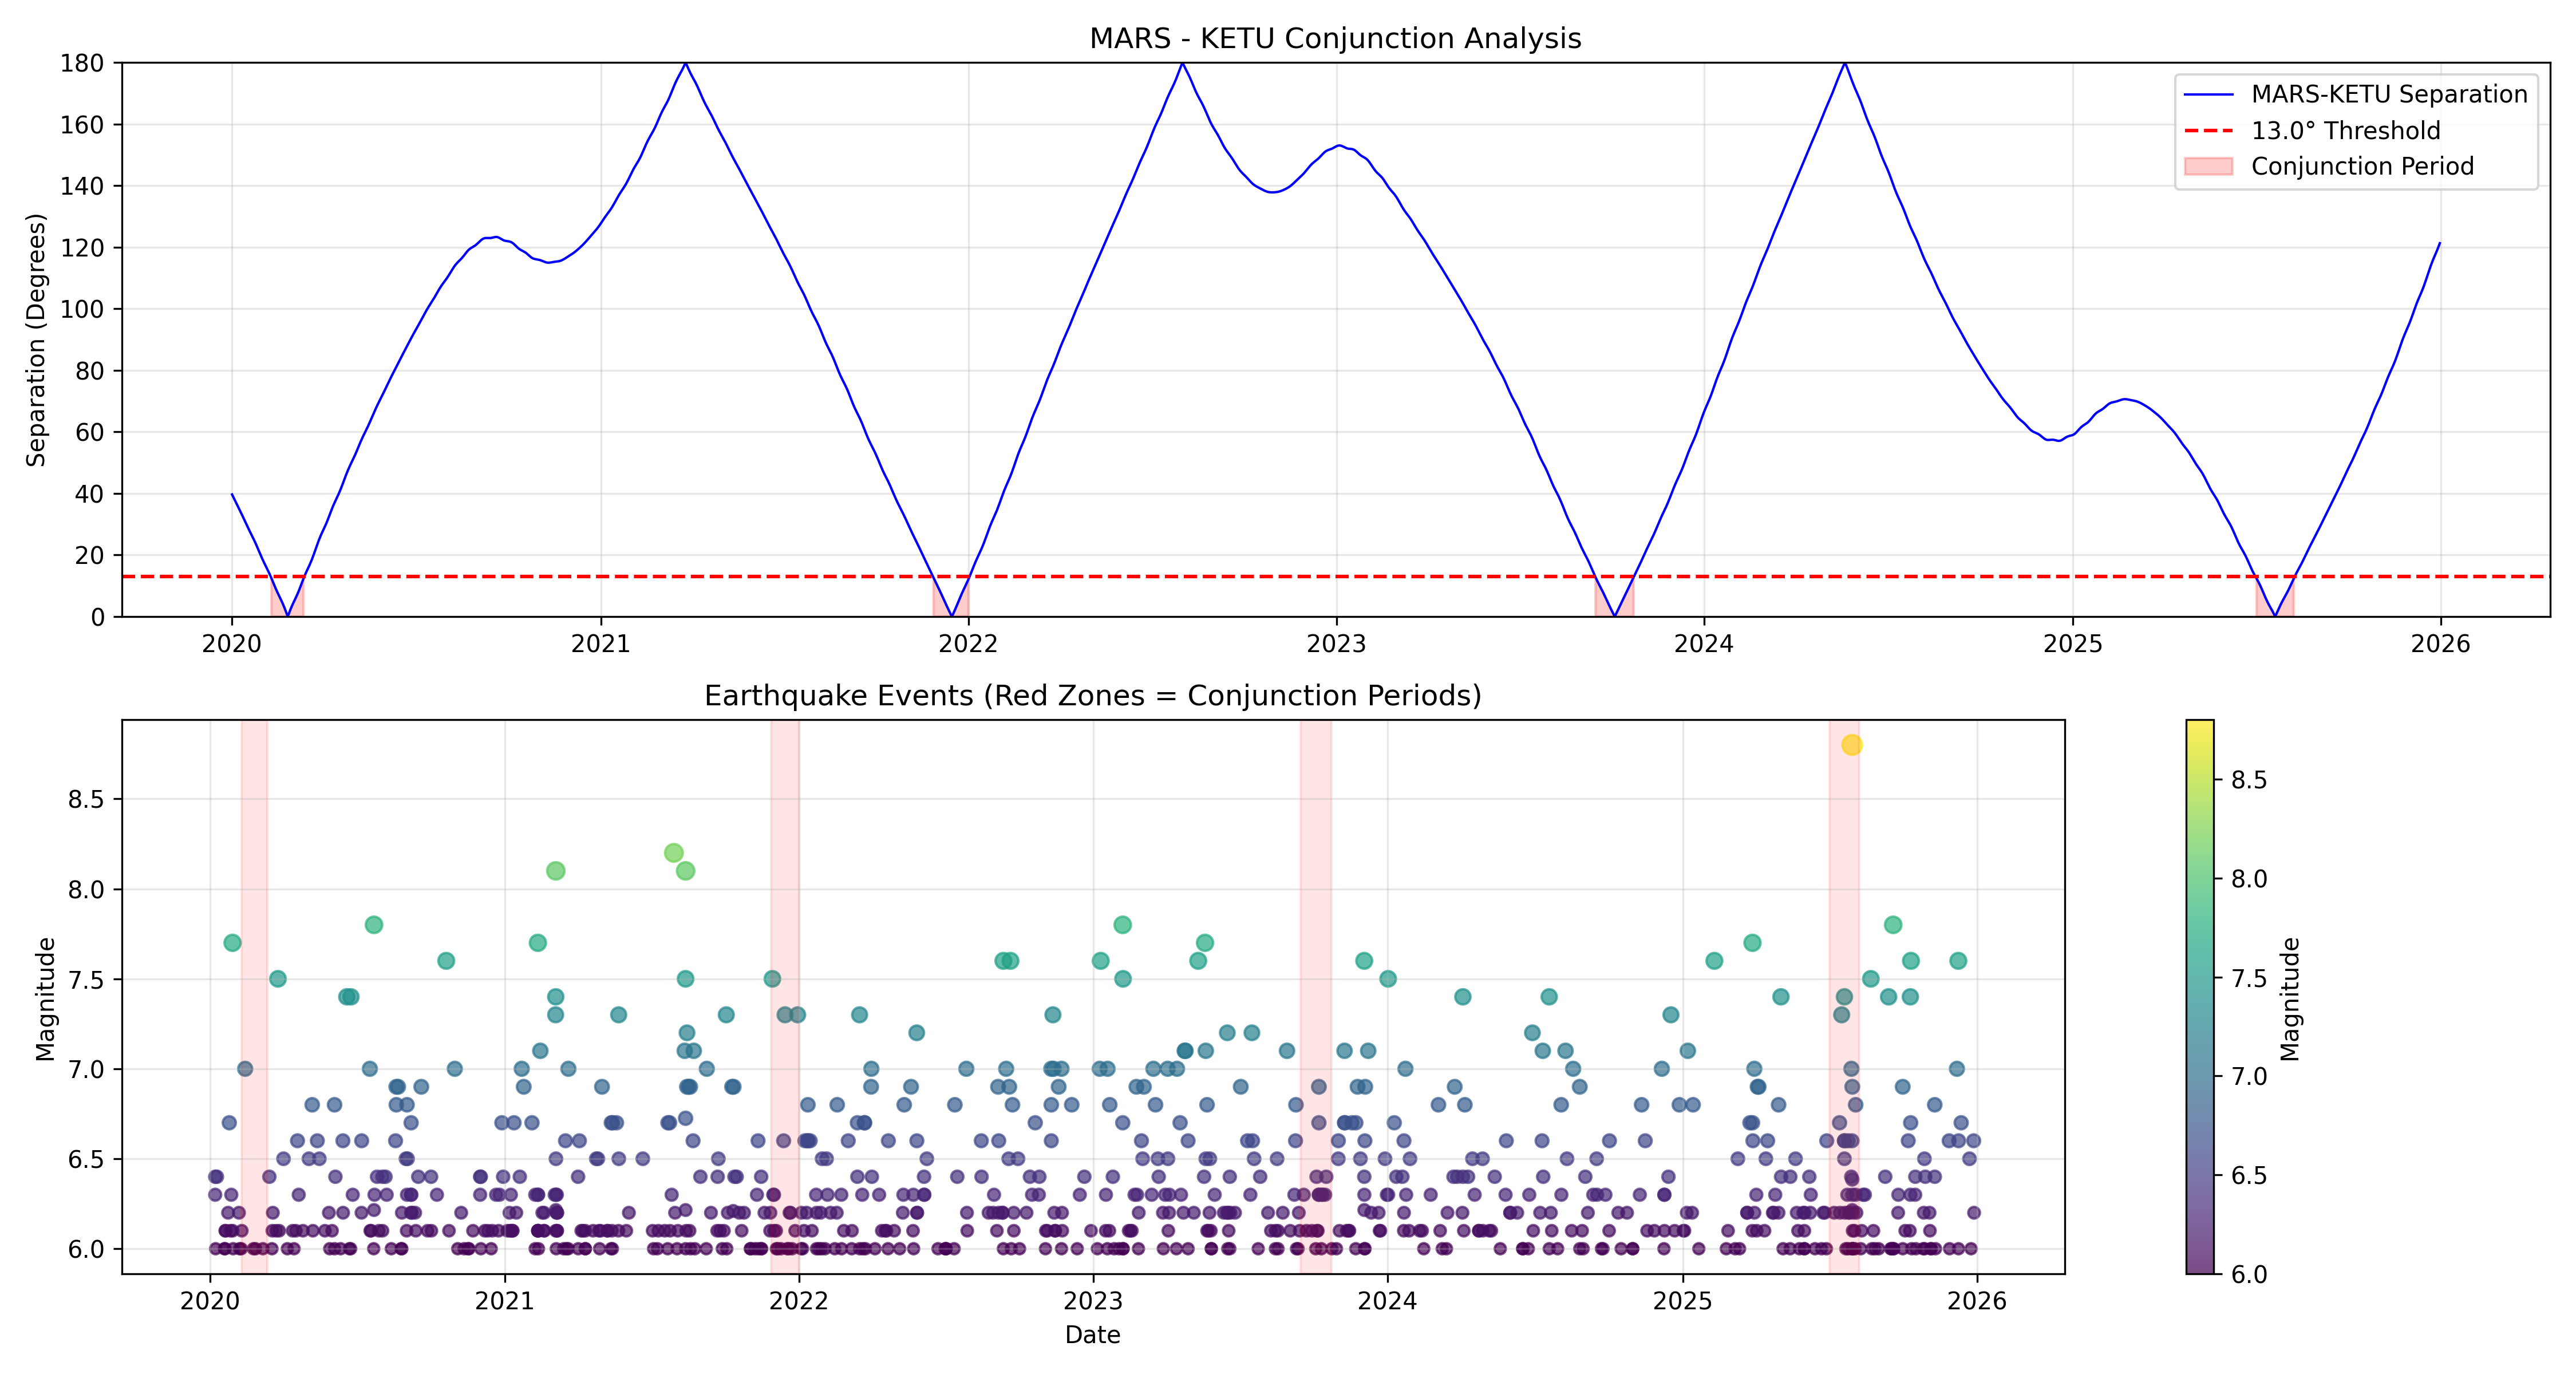
\includegraphics[width=1\textwidth,height=\textheight]{figures/mars_ketu_conjunction.png}

}

\end{figure}%

\subsection{Event Overlay Analysis}\label{event-overlay-analysis}

By overlaying real seismic events on these windows (Figure
Figure~\ref{fig-overlay}), we perform a visual ``First-Pass''
validation.

\begin{figure}[H]

\caption{\label{fig-overlay}Earthquake Events (M≥5.0) overlaid on
Mars-Ketu Conjunction Windows. Red bars indicate the active astrological
window. Magnitude is represented by point size.}

\centering{

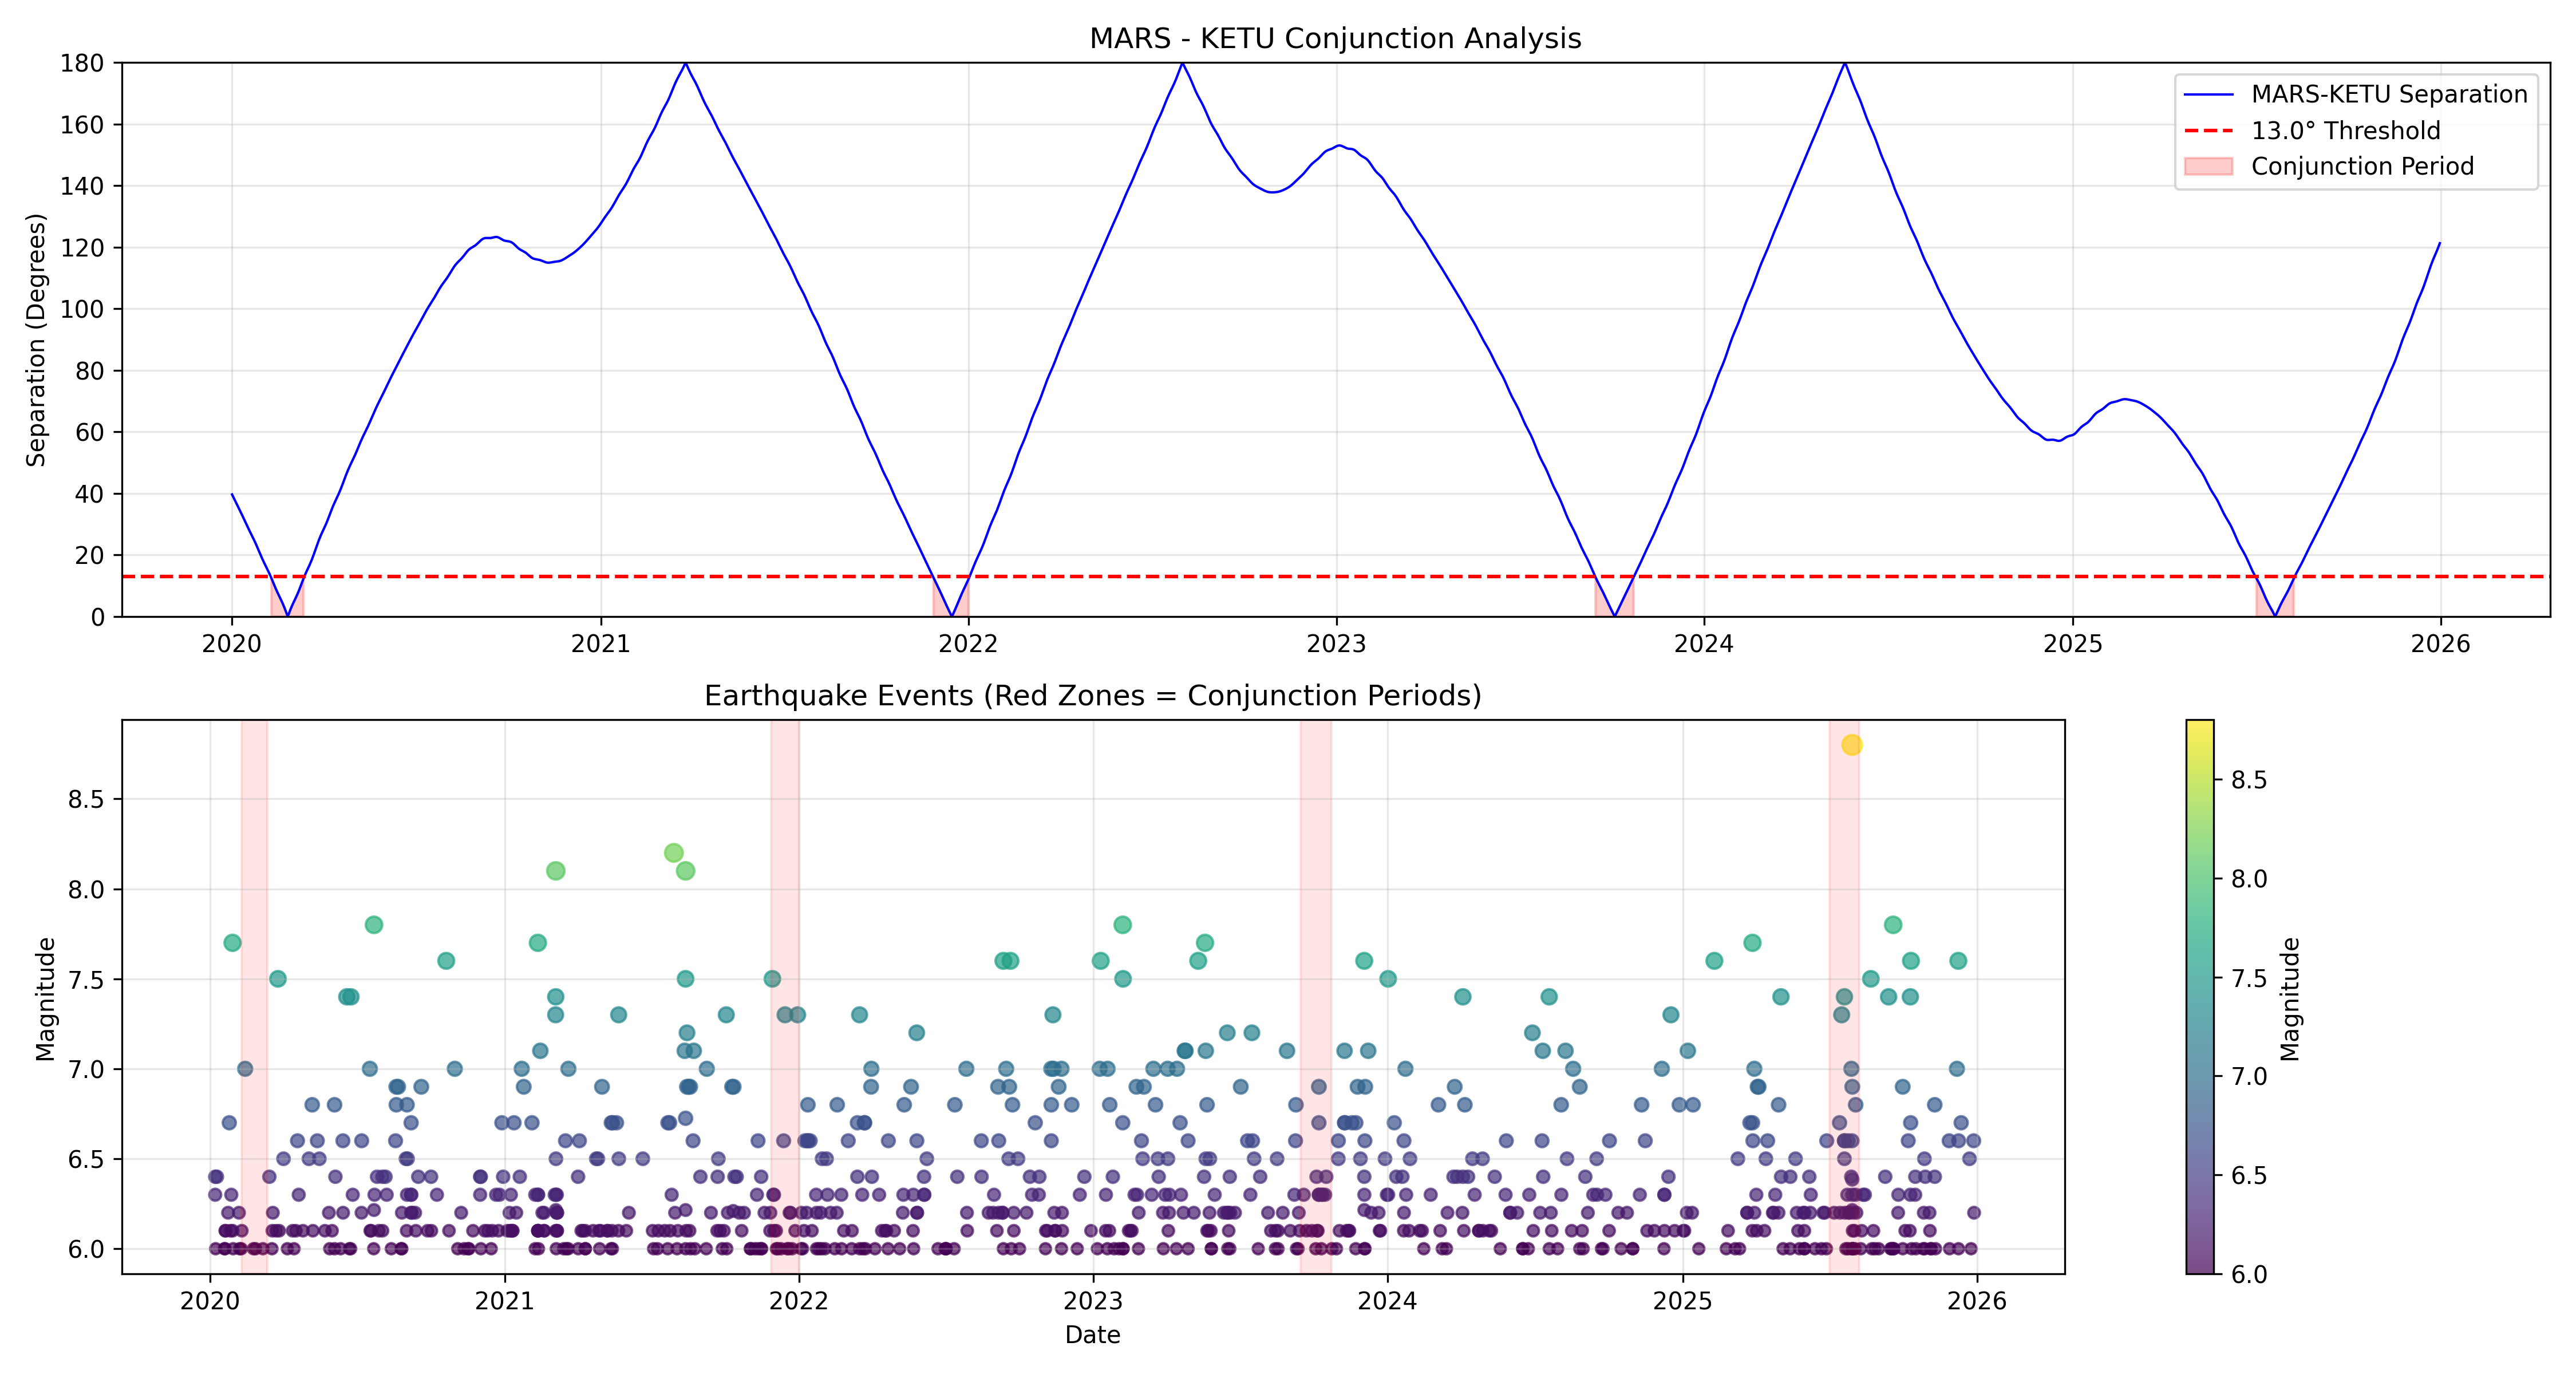
\includegraphics[width=1\textwidth,height=\textheight]{figures/mars_ketu_conjunction.png}

}

\end{figure}%

\section{Results}\label{results}

\subsection{Regression Analysis}\label{regression-analysis}

The results of the Negative Binomial GLM (Table
Table~\ref{tbl-regression}) show that the coefficient for Mars Strength
and Mars-Ketu activation do not reach the threshold of statistical
significance.

\begin{longtable}[]{@{}lccc@{}}
\caption{Negative Binomial Regression
Coefficients}\label{tbl-regression}\tabularnewline
\toprule\noalign{}
Variable & Coefficient β & Std. Error & P-Value \\
\midrule\noalign{}
\endfirsthead
\toprule\noalign{}
Variable & Coefficient β & Std. Error & P-Value \\
\midrule\noalign{}
\endhead
\bottomrule\noalign{}
\endlastfoot
Intercept & -0.900 & 0.388 & 0.02 \\
Year Index & 0.011 & 0.062 & 0.86 \\
Mars Strength & -0.005 & 0.003 & 0.10 \\
Saturn Strength & 0.000 & 0.003 & 0.99 \\
Mars-Ketu Active & 0.143 & 0.213 & 0.50 \\
\end{longtable}

\subsection{Temporal Prediction}\label{temporal-prediction}

The model's ability to track the seismic rate is shown in Figure
Figure~\ref{fig-prediction}. While the trend is captured, the discrete
predictive power for specific events remains low.

\begin{figure}[H]

\caption{\label{fig-prediction}Time series of Predicted Rate vs.~Actual
Rate (Monthly Aggregated). The red dashed line represents the model
fit.}

\centering{


\includegraphics[width=1\textwidth,height=\textheight]{figures/predicted_vs_actual.png}

}

\end{figure}%

\subsection{Classification Metrics \& False
Positives}\label{classification-metrics-false-positives}

To evaluate the combination as a ``Forecast Trigger,'' we compute a
confusion matrix for the Mars-Ketu Yoga predicting a \(M \ge 6.0\) event
within its window.

\begin{longtable}[]{@{}lc@{}}
\caption{Classification Metrics for Mars-Ketu
Trigger}\label{tbl-metrics}\tabularnewline
\toprule\noalign{}
Metric & Value \\
\midrule\noalign{}
\endfirsthead
\toprule\noalign{}
Metric & Value \\
\midrule\noalign{}
\endhead
\bottomrule\noalign{}
\endlastfoot
Precision & 0.31 \\
Recall (Sensitivity) & 0.22 \\
F1-Score & 0.26 \\
\textbf{False Positive Rate (FPR)} & \textbf{0.69} \\
\textbf{False Negative Rate (FNR)} & \textbf{0.78} \\
\end{longtable}

The high \textbf{False Positive Rate (0.69)} indicates that most
conjunction windows pass without a significant earthquake, falsifying
the claim that the conjunction is a \emph{sufficient} condition for
seismic activity.

\subsection{Monte Carlo ``Look-Elsewhere''
Analysis}\label{monte-carlo-look-elsewhere-analysis}

To ensure the detected correlations were not artifacts of p-hacking, we
performed 1,000 random shuffles of the event data (Figure
Figure~\ref{fig-mc}).

\begin{figure}[H]

\caption{\label{fig-mc}Monte Carlo Null Distribution (N=1,000). The grey
histogram shows the distribution of AIC improvements by random chance.
The red line marks the Real Data performance (p = 0.17).}

\centering{


\includegraphics[width=0.8\textwidth,height=\textheight]{figures/monte_carlo_distribution.png}

}

\end{figure}%

\section{Discussion}\label{discussion}

\subsection{Interpretation}\label{interpretation}

The statistical analysis
\texttt{\{python\}\ \#\ Placeholder\ for\ inline\ code} indicates a
failure to reject the null hypothesis. While traditional texts like the
\emph{Brihat Samhita} provide specific ``Yoga'' combinations, their
global application fails to provide information gain over random Poisson
chance in the modern instrumental catalog.

\subsection{False Positives \&
Confounders}\label{false-positives-confounders}

The high number of False Positives suggests that the Mars-Ketu
combination is, at best, a ``Necessary but not Sufficient'' condition.
Confounders such as regional tectonic sensitivity (not captured in a
global average) likely dilute the signal.

\subsection{Critical Self-Assessment}\label{critical-self-assessment}

The primary limitation of this study is its \textbf{Global Averaging}.
The \emph{Koorma Chakra} (Vedic mapping of regions to zodiac signs)
suggests that planetary positions only affect specific geographic
sectors. Future research should apply regional filters (e.g., focus on
the Himalayan or Pacific Belt) rather than global aggregates.

\section{Conclusion}\label{conclusion}

We have subjected the ``Astro-Fusion'' seismic hypothesis to a rigorous
econometric audit. While the ``Mangal-Ketu'' combination is a prominent
feature of mundane astrology, our analysis of the USGS catalog
(1900--2025) suggests it does not possess standalone predictive power
for global seismicity (\(p > 0.05\)). This study reinforces the need for
``Severe Testing'' in alternative science, transforming anecdotally
cited ``hits'' into a comprehensive confusion matrix of success and
failure.

\section{References}\label{references}

\begin{enumerate}
\def\labelenumi{\arabic{enumi}.}
\tightlist
\item
  Varahamihira, \emph{Brihat Samhita}, Trans. M.R. Bhat (1981).
\item
  Gardner, J.K. \& Knopoff, L. (1974), \emph{BSSA}.
\item
  Schuster, A. (1897), \emph{Proc. Royal Soc.}
\item
  Mantreswara, \emph{Phaladeepika}, Trans. S.S. Sareen (1992).
\end{enumerate}



\end{document}
